\documentclass{article}

\usepackage{Sweave}
\begin{document}
\Sconcordance{concordance:teste.tex:teste.Rnw:%
1 2 1 1 0 9 1 1 12 4 0 1 2 1 4 1 2 1 1 1 3 5 0 1 2 2 1}






\section{TESTE}


\begin{Schunk}
\begin{Soutput}
[1] ":- set(classes,[no,yes]).\n% :- set(tree_type,classification).\n:- set(tree_type,class_probability).\n:- set(minpos,10).  % minimum examples in leaf for splitting\n:- set(clauselength,50).\n:- set(lookahead,2).\t% to allow lookahead to lteq/2\n:- set(prune_tree,true).\n:- set(confidence,0.25).% pruning conf parameter used by C4.5\n:- set(evalfn,entropy).\n% :- set(evalfn,gini).\n:- set(dependent,2)."
\end{Soutput}
\end{Schunk}

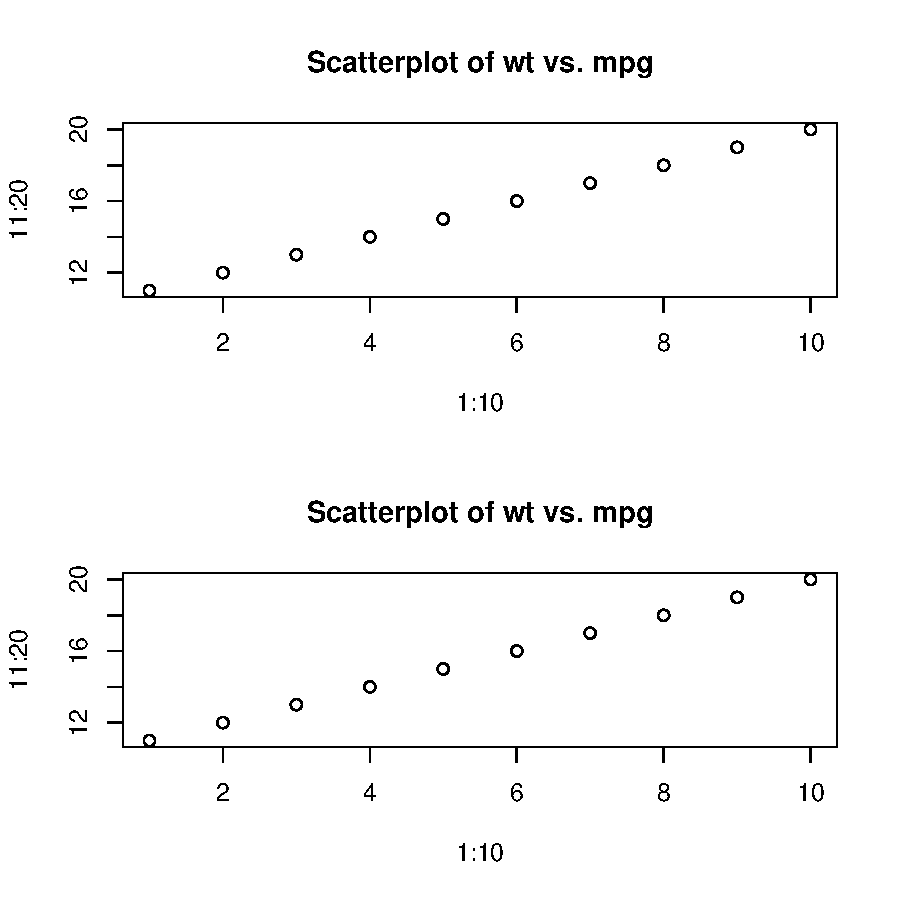
\includegraphics{teste-002}


\begin{Schunk}
\begin{Soutput}
[1] "sdff"
[1] "sdff"
\end{Soutput}
\end{Schunk}


\end{document}
